\documentclass[a4paper, 12pt]{article}
\usepackage[UTF8]{ctex}
% \usepackage[T1]{fontenc}
% \usepackage{inconsolata}

\usepackage[hidelinks]{hyperref}

\usepackage{amsmath}
\usepackage{enumitem}
\setlist{
    nolistsep, % 去掉 item 和正文之间的间隔
    % labelindent=\parindent,
    leftmargin=*, % 保证小节标签缩进和上面对齐
    % labelsep=1em, % 标签后的空白
    align=left, % 标签对齐段落左边缘
}
\usepackage{tabularx}

\usepackage{graphicx}
\usepackage{subfig}
% \usepackage{subcaption}

\usepackage{geometry}
\geometry{
    a4paper,
    left=2cm,
    right=2cm,
    top=2cm,
    bottom=2cm,
}

\newcommand{\fs}[1]{\fontsize{#1 pt}{0pt}\selectfont}

\usepackage{mathtools}
\DeclarePairedDelimiter{\ceil}{\lceil}{\rceil}
\DeclarePairedDelimiter\floor{\lfloor}{\rfloor}

\usepackage{setspace}
% \setlength\parindent{0pt}
\setlength{\parindent}{2em} % 中文

% \newfontfamily\csl{Consolas}

\usepackage{array}
\newcolumntype{T}{>{\ttfamily}l}
\newcolumntype{Y}{>{\footnotesize\ttfamily}l}
\newcolumntype{y}{>{\footnotesize\ttfamily}c}

\usepackage{longtable}

\newcommand*{\thead}[1]{\multicolumn{1}{c}{\bfseries #1}}
\newcommand*{\yhead}[1]{\multicolumn{1}{c}{\footnotesize\bfseries #1}}

\newcommand{\ssa}{\phantom{x}}
\newcommand{\ssb}{\phantom{xx}}
\newcommand{\ssc}{\phantom{xxx}}
\newcommand{\ssd}{\phantom{xxxx}}
\newcommand{\sse}{\phantom{xxxxx}}

\usepackage{xcolor}
\usepackage{listings}
\definecolor{mygreen}{RGB}{28,172,0} % color values Red, Green, Blue
\definecolor{mylilas}{RGB}{170,55,241}

\newcommand{\ttf}{\ttfamily}

\lstdefinestyle{plainText}{language={},
    basicstyle=\footnotesize \ttfamily,        % set font type and size
    % basicstyle=\ttfamily,        % set font type and size
    breaklines=true,
    keywordstyle=\color{blue},
    % morekeywords={matlab2tikz},
    % morekeywords=[2]{1}, 
    % keywordstyle=[2]{\color{black}},
    identifierstyle=\color{black},
    stringstyle=\color{mylilas},
    % stringstyle=\color{purple},
    frame=single,
    framexleftmargin=0em,
    aboveskip=-\baselineskip,
    commentstyle=\color{mygreen},
    showstringspaces=false,% without this there will be a symbol in the places where there is a space
    % numbers=left,
    numbers=none,
    numberstyle={\tiny \color{black}}, % size of the numbers
    numbersep=9pt, % this defines how far the numbers are from the text
    tabsize=4,                     % sets default tabsize to 4 spaces
    emph=[1]{},
    emphstyle=[1]\color{blue}, %some words to emphasise
    %emph=[2]{word1,word2}, 
    % emphstyle=[2]{style}, 
    escapeinside=``,               % Characters escape: To Use Chinese in codes   
}

\lstdefinestyle{myC}{language={C},
    % basicstyle=\footnotesize \ttfamily,        % set font type and size
    basicstyle=\ttfamily,        % set font type and size
    breaklines=true,
    keywordstyle=\color{blue},
    % morekeywords={matlab2tikz},
    % morekeywords=[2]{1}, 
    % keywordstyle=[2]{\color{black}},
    identifierstyle=\color{black},
    stringstyle=\color{mylilas},
    % stringstyle=\color{purple},
    frame=single,
    framexleftmargin=0em,
    aboveskip=-\baselineskip,
    commentstyle=\color{mygreen},
    showstringspaces=false,% without this there will be a symbol in the places where there is a space
    % numbers=left,
    numbers=none,
    numberstyle={\tiny \color{black}}, % size of the numbers
    numbersep=9pt, % this defines how far the numbers are from the text
    tabsize=4,                     % sets default tabsize to 4 spaces
    emph=[1]{function, return, f, let, add, mult, dot, rk, uw2uwdd, uw2xy1, uw2xy2},
    emphstyle=[1]\color{blue}, %some words to emphasise
    % emph=[2]{word1,word2}, 
    % emphstyle=[2]{style}, 
    escapeinside=``,               % Characters escape: To Use Chinese in codes   
}


\lstdefinestyle{myPython}{language=Python,
    % basicstyle=\footnotesize \ttconsolas,        % set font type and size
    basicstyle=\footnotesize \ttfamily,        % set font type and size
    breaklines=true,
    keywordstyle=\color{blue},
    % morekeywords={matlab2tikz},
    % morekeywords=[2]{1}, 
    % keywordstyle=[2]{\color{black}},
    identifierstyle=\color{black},
    stringstyle=\color{mylilas},
    % stringstyle=\color{purple},
    frame=single,
    framexleftmargin=0em,
    aboveskip=-\baselineskip,
    commentstyle=\color{mygreen},
    showstringspaces=false,% without this there will be a symbol in the places where there is a space
    numbers=left,
    numberstyle={\tiny \color{black}}, % size of the numbers
    numbersep=9pt, % this defines how far the numbers are from the text
    tabsize=4,                     % sets default tabsize to 4 spaces
    emph=[1]{nonLinearFunction, bitReorganization, modAdd_2e31m1, binaryAdd, binaryXor, sboxOfZuc, linearTransform},
    emphstyle=[1]\color{red}, %some words to emphasise
    %emph=[2]{word1,word2}, 
    % emphstyle=[2]{style}, 
    escapeinside=``,               % Characters escape: To Use Chinese in codes   
}


\begin{document}

\begin{center}
{\fs{15}\bfseries {神经网络与机器学习~作业~1~报告}}

{\fs{13}\bfseries {红外图像数据的聚类}}

\vspace{0.5\baselineskip}

{\fs{14} \kaishu 于泽汉 \hspace{1em} \textsf{No.118039910141}}
\end{center}


\section{题目}

查阅相关文献,根据所给红外图像数据集,实现一种分类或聚类方法。

作业要求:
\begin{enumerate}[leftmargin=*,labelindent=2em]
\item 模型建立和理论求解过程。例如,数据的处理方式?求解方法的选择?参数的控制和调节?方法讨论等。 
\item代码实现过程:原始代码+代码注释+结果展示,需说明运行平台。
\item 附参考文献。
\end{enumerate}


\section{摘要}
本实验对所给红外图像数据集进行了预处理,并从处理后的图像中提取相关特征,利用这些特征,对拍摄的不同场景下的红外图像进行聚类。


\section{问题描述}

给定一组不同场景下的红外图像数据集,需要将不同场景下的图像划分到不同的类中。

需要尽可能实现如下目标:

\begin{enumerate}[leftmargin=*,labelindent=2em]
\item 聚类效果好,能将所有不同类型的图像都区分开来。
\item 聚类方法简单实用,减少不必要的麻烦,降低出错的可能性。
\item 聚类速度快,效率高,可以处理大量的数据。
\end{enumerate}

\section{模型建立过程}

首先,需要将所给的红外图像转换成合适的格式与形式,方便进行后续的分析和处理。这里需要对一些常用的格式转换流程和图像处理方式作一定的了解。

其次,不同的图像预处理方法,会对图像的特征提取产生较大的影响。因此需要针对目标图像的特点选择合适的预处理方法,以突出不同类型图像的特征。

再者,选取不同的特征,对不同类型图像的区分程度不同。所以需要尝试各种特征,并且合理地选取维数,从而用尽可能少的维度产生尽可能大的区分度。

最后,采用不同的聚类方法,聚类效果也不一样。一般倾向于先采用简单的方法,如果效果较好,那么万事大吉,如果效果不好,可以适当调整参数以改善效果,或者向上回溯修改提取的特征、采用的维数甚至是预处理方法,或者是采用新的聚类方法。

\section{模型求解过程}

\subsection{图像预处理}
首先,所给的图像如果不加处理,那么在聚类时就会出现误差,从而影响聚类的结果。

比如图 \ref{fig:a} 中的两张图像,飞机在不同时刻面对太阳的方向不同,因此机身的明暗发生了变化。如果只是提取图像中的明暗关系,那么这两张图就有可能被分到两个不同的类中。

\begin{figure}[htbp]
    \centering
    \subfloat[机身向光(亮)]{%
        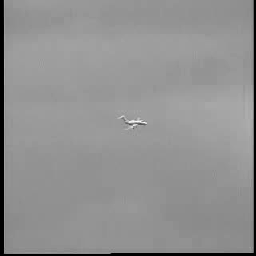
\includegraphics[width=0.35\textwidth]{./images/A_light.png}}
    \phantom{123}
    \subfloat[机身背光(暗)]{%
        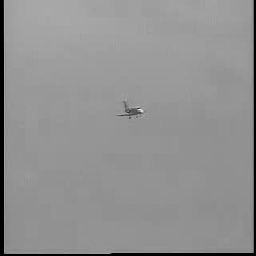
\includegraphics[width=0.35\textwidth]{./images/A_dark.png}}\\
    \caption{同一个场景下(因此应属同一类)的两张图像有明暗的变化}
    \label{fig:a}
\end{figure}

实际实验中,也确实发现,只利用灰度的均值或方差,对图像进行聚类的效果并不好,尤其是明暗发生变化的这两组图像。

因此考虑对图像进行\textbf{灰度化}和\textbf{锐化}。

灰度化将 RGB 的三维色彩值转换成一维的灰度值,减少图像处理的工作量。

而锐化则采用 Sobel 算法。该算法通常用于边缘检测,这里用于滤掉图像的明暗差异,而保留边缘和轮廓的信息。

上面两幅图像锐化后的结果如图 \ref{fig:sobel} 所示。

\begin{figure}[htbp]
    \centering
    \subfloat[机身向光(亮)(锐化后)]{%
        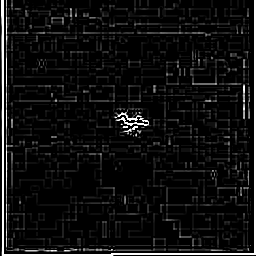
\includegraphics[width=0.35\textwidth]{./images/A_light_x.png}}
    \phantom{123}
    \subfloat[机身背光(暗)(锐化后)]{%
        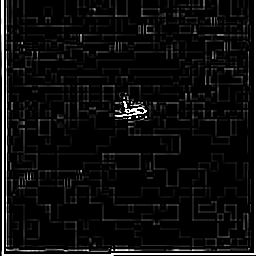
\includegraphics[width=0.35\textwidth]{./images/A_dark_x.png}}\\
    \caption{图像锐化后,明暗的影响被消除,边缘和轮廓的信息得到保留}
    \label{fig:sobel}
\end{figure}

对数据集中的其他图像也都作同样的灰度化和锐化处理。

\subsection{选取特征}
一张图像中蕴含的信息极多,因此如何用最少的维度来区分不同的图像,是一个需要仔细思考的问题。考虑到这次实验中所给图像相互之间的区别较大,因此选取比较常用的特征应该就可以实现比较好的聚类效果。

经过思索和尝试,最终选取图像中所有像素点灰度值的\textbf{均值}和\textbf{方差}这两个维度,作为聚类时输入的向量。

因此,需要采取的操作如下:

\begin{enumerate}[leftmargin=*,labelindent=2em]
\item 将每一张图像分别转换成一个二维数值矩阵,矩阵中每个元素的值就是该像素点的灰度值。
\item 计算每一个二维数值矩阵中全体元素的均值和方差,并进行归一化。
\item 将每一组均值和方差化成二维向量,形成向量组,作为后续聚类的输入。
\end{enumerate}


\subsection{进行聚类}
有很多可供选用的聚类算法,不过 $k$-means 算法应该是其中最为简单和高效的一种了。

越是简单的东西,实现越容易,也就越不容易出错。由于本次的图像数据比较友好,因此使用 \textbf{$\mathbf{k}$-means} 算法就足以满足我们的要求。

所以此次实验将二维向量(均值和方差)作为空间中的点,来对这些点进行聚类。

本次实验采用的聚类的流程和一般的 $k$-means 算法几乎没有差别,除了\textbf{对初始化一步进行了优化}。

一般的 $k$-means 算法在初始化时是随机选取 $k$ 个中心点的,而不同的初始中心会对后续的收敛速度和聚类结果产生很大的影响。此处作的优化就是,在选取初始点时,尽可能选取空间距离较大的那些点,从而提高收敛的速度和聚类结果的准确度。

还有一个需要注意的是 $k$ 值的选取。由于此次实验比较容易看出类的数目,因此可以直接指定 $k$ 值。对于更广泛或者是不确定类数目的情况,还需要选取适当的指标和自动化的迭代流程,来保证选到最合适的 $k$ 值。

\section{代码实现}
限于篇幅,这里略去了部分细节,完整的代码请见附件。

重命名文件这一步对算法本身没有作用,只是为了后面方便对比聚类结果和真实结果。

\begin{lstlisting}[style=myPython,caption={重命名文件}]
src = "data/"
dst = "data_renamed/"
tgt = "data_processed/"

def renameFiles():
    if not os.path.exists(dst): 
        os.mkdir(dst)
    for filename in os.listdir(src):
        name, ext = os.path.splitext(filename)
        print(name)
        if ext == ".bmp":
            cls = "A"
        elif ext == ".png":
            cls = "B"
        elif ext == ".jpg":
            if name == "timg":
                cls = "D"
            else:
                cls = "C"
        else:
            cls = "X"
        copyfile(src+filename,dst+cls+filename)
\end{lstlisting}

首先对图像进行预处理,主要是灰度化和锐化。这里使用了 Sobel 算子,当然也可以用 Scharr 算子或者 Laplacian 算子,得到的结果大同小异。这里需要注意图像的格式和编码。

\begin{lstlisting}[style=myPython,caption={图像的灰度化和锐化}]
imgs = []
def sharpImages():
    if not os.path.exists(tgt): 
        os.mkdir(tgt)
    global imgs
    for filename in os.listdir(dst):
        tmp = cv2.imread(dst+filename,0)
        res = cv2.Sobel(tmp, cv2.CV_64F,1,1, ksize=5)
        # res = cv2.Laplacian(tmp,cv2.CV_64F,ksize=5)
        # res = cv2.Scharr(tmp,cv2.CV_64F,1,0)
        imgs.append([res,filename])
        cv2.imwrite(tgt+filename,res)
\end{lstlisting}

接下来是计算每个数值矩阵中所有元素的均值和方差,归一化后将其转换成二维向量。这里依旧需要注意各种数据类型和格式的匹配。

\begin{lstlisting}[style=myPython,caption={计算每个数值矩阵中所有元素的均值和方差}]
means = []
varis = []
names = []
colors = ['red', 'green', 'blue', 'black', 'cyan']
types = ['A','B','C','D','E']
def extractFeatures():
    global imgs
    imgs = []
    for filename in os.listdir(tgt):
        pix = cv2.imread(tgt+filename)
        imgs.append([pix,filename])
    global means, varis, names
    plt.figure(0)
    for img in imgs:
        pix = img[0]
        means.append(np.sum(np.absolute(pix))/pix.size)
        varis.append(np.std(pix))
        names.append(img[1])

        filename = img[1]
        plt.plot(means[-1],varis[-1], marker='o',color=colors[types.index(filename[0])])
    means = np.array(means)
    varis = np.array(varis)
    [means, varis] = list(map(lambda x: np.interp(x, (x.min(),x.max()),(0,10)), [means, varis]))
\end{lstlisting}

最后是使用 $k$-means 算法进行聚类。相比一般的 $k$-means 算法,这里对初始化步骤进行了改进。这个部分是最复杂也是最容易出错的,一定要想清楚之后再动手。

\begin{lstlisting}[style=myPython,caption={使用 $k$-means 算法进行聚类}]
def clusterImages(k):
    n = len(means)
    mv = []
    for idx in range(0,n):
        mv.append(np.array([means[idx],varis[idx]]))
    visited = []
    clusters = [[] for _ in range(k)]
    ## Initialize centers
    clusters[0].append(random.randint(0,n-1))
    visited.append(clusters[0][0])
    tmpCenter = np.array(mv[0])
    for i in range(1,k):
        maxDist = 0
        cenIdx = -1
        for j in range(0,n):
            if j in visited:
                pass
            else:
                tmpDist = np.linalg.norm(mv[j]-tmpCenter)
                if tmpDist>maxDist:
                    maxDist = tmpDist
                    cenIdx = j
        clusters[i].append(cenIdx)
        visited.append(cenIdx)
        tmpCenter = (tmpCenter*i + mv[clusters[i][0]])/(i+1)
    centers = []
    centersOld = []
    for i in range(0,k):
        centers.append(mv[clusters[i][0]])
    ## Clustering
    isClustered = False
    epoch = 0
    while not isClustered:
        if epoch==0:
            pass
        else:
            visited = []
            clusters = [[] for _ in range(k)]
        print(epoch)
        epoch += 1

        for j in range(0,n):
            if j in visited:
                pass
            else:
                minDist = float("inf")
                clsIdx = -1
                for i in range(k):
                    tmpDist = np.linalg.norm(mv[j]-centers[i])
                    if tmpDist < minDist:
                        minDist = tmpDist
                        clsIdx = i
                clusters[clsIdx].append(j)
        ## Check is clustered
        if len(centersOld) == 0:
            centersOld = centers.copy()
            continue
        else:
            isClustered = True
            for i in range(0,k):
                centerTmp = np.array([0,0])
                for idx in clusters[i]:
                    centerTmp = centerTmp + mv[idx]
                centers[i] = centerTmp/len(clusters[i])
                isClustered = isClustered and (centers[i][0]==centersOld[i][0]) and (centers[i][1]==centersOld[i][1])
            print(isClustered, list(map(lambda i: (round(centers[i][0],3),round(centers[i][1],3)), [0,1,2,3])))
            centersOld = centers.copy()
    plt.figure(1)
    for i in range(len(clusters)):
        for j in range(0,len(clusters[i])):
            tmpX = mv[clusters[i][j]][0]
            tmpY = mv[clusters[i][j]][1]
            # print(i,j,mv[clusters[i][j]])
            plt.plot(tmpX,tmpY,marker="o",color=colors[i])
    plt.show()
\end{lstlisting}

主函数用于依次执行上述流程。

\begin{lstlisting}[style=myPython,caption={主函数}]
if __name__ == '__main__':
    renameFiles()
    sharpImages()
    extractFeatures()
    clusterImages(4)
\end{lstlisting}

\section{结果与分析}
聚类得到的结果如图 \ref{fig:result} 所示。

左图是图像数据实际所属的类别,用不同的颜色加以区分。右图是聚类得到的图像所属的类别。需要注意的是,左图和右图中的颜色并无关联,不同的颜色仅用于区分不同的类,并不是对应到具体的类。另外,右图中的横纵坐标也都是“归一化”了的(数值重映射到 $[0,10]$ 的范围)。

从图中可以看出,聚类效果非常好,不同的类间隔明显,同类的数据点则相距紧密。右上角单独的一个点,也确实是数据集中唯一一张单独成类的图像,换句话说,实现的算法对异常值的容忍度和辨识度也是非常高的。

\begin{figure}[htbp]
    \centering
    \subfloat[图像数据实际的类别]{%
        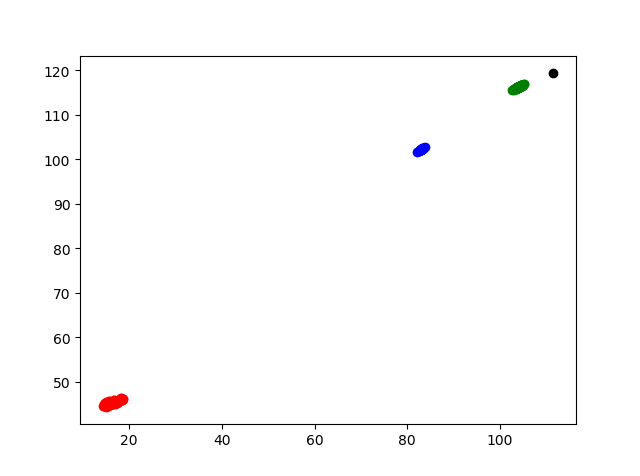
\includegraphics[width=0.45\textwidth]{./images/original.png}}
    \phantom{123}
    \subfloat[算法实现得到的聚类]{%
        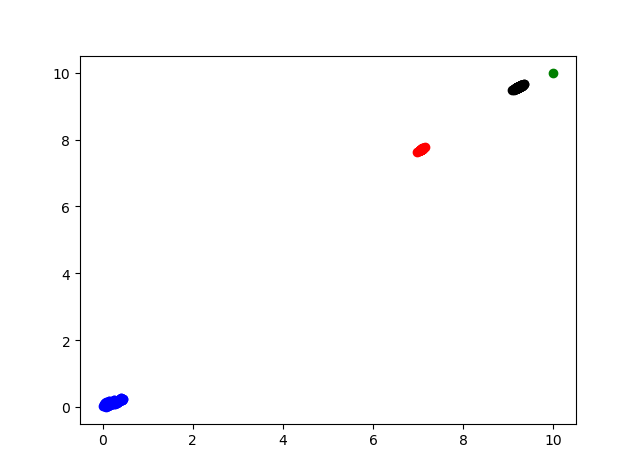
\includegraphics[width=0.45\textwidth]{./images/clustered.png}}\\
    \caption{算法将属于不同类别的图像准确地分开了}
    (此处不同的颜色仅用于区分不同的类,并不是对应到具体的类)
    \label{fig:result}
\end{figure}

\newpage
算法的输出如下所示。该输出的含义是,算法只进行了 3 次迭代就成功完成了聚类。方括号中的内容是,每次迭代后各个类的中心点坐标。为了使结果显得整洁,在输出时取了有效位数,实际算法中使用的是较高精度的数值。可以看到第 3 次迭代时的中心点相比第 2 次没有发生变化,表示各个中心已经稳定,因此迭代终止,完成聚类。

\begin{itemize}[label={},leftmargin=2em]
\item \begin{lstlisting}[style=plainText,caption={算法的输出}]
0

1
False [(8.637, 9.073), (10.0, 10.0), (0.211, 0.127), (9.273, 9.612)]
2
False [(7.065, 7.71), (10.0, 10.0), (0.211, 0.127), (9.224, 9.578)]
3
True [(7.065, 7.71), (10.0, 10.0), (0.211, 0.127), (9.224, 9.578)]
\end{lstlisting}
\end{itemize}

图 \ref{fig:zoom} 放大展示了上面右图中左下角的一类。从图中可以看出,尽管在图 \ref{fig:result} 中同类的点看上去好像非常紧密,但实际上它们也是分布在一定范围内的,同类中的不同图像的特征也是存在微小差异的。这一结果也从侧面印证了我们实现的算法是能够准确地分出同类和不同类的图像的。

\begin{figure}[htbp]
    \centering
    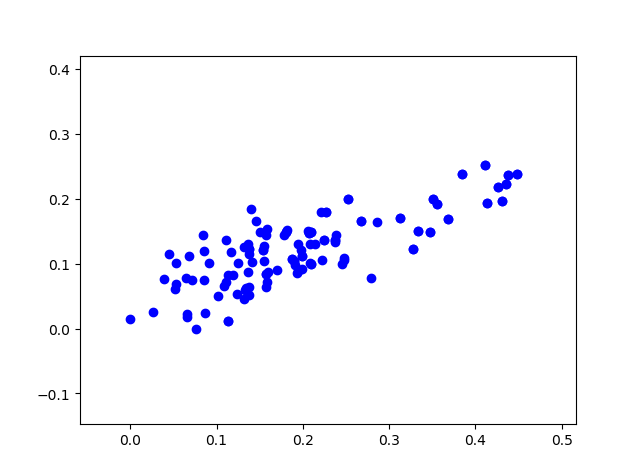
\includegraphics[width=0.8\textwidth]{./images/clustered_zoom.png}
    \caption{同一类中不同图像对应的点在该空间中的分布}
    \label{fig:zoom}
\end{figure}

实际上,除了使用 $k$-means 算法,此次实验中的数据集也可以使用 DBSCAN 算法。不过 DBSCAN 的复杂度比 $k$-means 更高,并且由于 $k$-means 对于此次所给数据集已经足够好用,因此在时间和资源有限的情况下,还是倾向于使用 $k$-means 算法,以减少不必要的麻烦。只有效果始终调整不好的情况下,才应该用更加复杂的算法。

\section{参考文献}

\begin{enumerate}
\item Wikipedia contributors. (2019, May 6). K-means clustering. In Wikipedia, The Free Encyclopedia. Retrieved 16:23, May 9, 2019, from \url{https://en.wikipedia.org/w/index.php?title=K-means_clustering&oldid=895778515}
\item Wikipedia contributors. (2019, April 18). DBSCAN. In Wikipedia, The Free Encyclopedia. Retrieved 16:38, May 9, 2019, from \url{https://en.wikipedia.org/w/index.php?title=DBSCAN&oldid=893049545}
\item Wikipedia contributors. (2019, April 3). Edge detection. In Wikipedia, The Free Encyclopedia. Retrieved 16:39, May 9, 2019, from \url{https://en.wikipedia.org/w/index.php?title=Edge_detection&oldid=890804463}
\item Wikipedia contributors. (2019, February 1). Sobel operator. In Wikipedia, The Free Encyclopedia. Retrieved 16:27, May 9, 2019, from \url{https://en.wikipedia.org/w/index.php?title=Sobel_operator&oldid=881233268}
\item Stéfan van der Walt, S. Chris Colbert and Gaël Varoquaux. The NumPy Array: A Structure for Efficient Numerical Computation, Computing in Science \& Engineering, 13, 22-30 (2011), DOI:10.1109/MCSE.2011.37
\end{enumerate}

\end{document}